\chapter{Implementierung der Polynome}

Die Implementierung der einzelnen Bestandteile ist objektorientiert. Dieses Kapitel bietet einen Überblick über die Struktur des Programmes und den wichtigsten zu Verfügung stehenden Funktionen.

\section{Darstellung}

\paragraph{Intervalle}
Intervalle enthalten Informationen über deren Zentrum \verb+center+ und Radius \verb+radius+, beziehungsweise deren Breite, welche, je nach gewähltem Zahlentypen, reelle oder rationale Zahlen sind. Zudem können Intervalle ein- oder beidseitig unendlich sein, weshalb wiederum eine Abfrage nach \verb+IntType+\footnote{ FINITE, LOWER\_BOUND, UPPER\_BOUND, ENTIRE }, also dem Intervalltypen möglich ist. Existiert eine Schranke, also ist das Intervall endlich oder einseitig unendlich, kann diese abgefragt werden. \par
Beim Verrechnen von Intervallen sind folgende Regeln zu beachten:
\begin{itemize}
    \item[] $[x_1, x_2] + [y_1, y_2] = [x_1 + y_1, x_2 + y_2]$
    \item[] $[x_1, x_2] - [y_1, y_2] = [x_1 - y_2, x_2 - y_1]$
    \item[] $[x_1, x_2] \cdot [y_1, y_2] = [min(x_1 y_1, x_1 y_2, x_2 y_1, x_2 y_2), max(x_1 y_1, x_1 y_2, x_2 y_1, x_2 y_2)]$
    \item[] $[x_1, x_2] / [y_1, y_2] = [min(x_1 / y_1, x_1 / y_2, x_2 / y_1, x_2 / y_2), max(x_1 /y_1, x_1 /y_2, x_2 /y_1, x_2 /y_2)]$
\end{itemize}
Hier wird der Effekt deutlich, dass Intervalle nach jeder Operation die Tendenz haben, zu wachsen. Wird  bespielsweise ein Intevall  von sich selbst subtrahiert, wird es größer, statt sich wegzukürzen.



\paragraph{Fehlersymbole} 
Ein Fehlersymbol $\lambda$ besteht aus seinem Exponenten, einem \verb+Pointer+ auf das Intervall in dem sein Wert liegt, welches sich während der Berechnung verändern kann und dem Index des Fehlersymbols.

\paragraph{Monome}
Momome werden durch einen Intervallkoeffizienten und eine Liste von nach ihrem Index aufsteigend geordneten Fehlersymbolen dargestellt. Die Implementierung der Liste der Fehlersymbole als \verb+std::vector+, ermöglicht die Verwendung der \textit{C++ Standard Template Library} für Funktionen, wie zum Beispiel die Berechnung des Grades eines Monoms.

\paragraph{Polynome}
Ein Polynom setzt sich aus einem Kernintervall (\verb+kernel+), also dem Monom ohne Fehlersymbole und einer Liste ungleicher Monome zusammen. Ungleich bedeutet in diesem Fall, dass sich die Zusammensetzung  oder der Exponent einzelner Fehlersymbole zwischen den Monomen unterscheidet.


\section{Addition}

Wird wie in \cite{geobuckets} eine Ordnung $\succ$ auf den Monomen definiert, können die Polynome sortiert werden.
\begin{itemize}
    \label{def:order}
    \item $\lambda_1 \succ \lambda_2 \succ...\succ \lambda_k $
    \item $\lambda_n^i \lambda_m^j \succ \lambda_n^{i'} \lambda_m^{j'} $ für $n > m$, falls
    \begin{itemize}
        \item[] $ i > i'$, oder
        \item[] $ i = i'$ und $ j > j'$
    \end{itemize}
\end{itemize}
Diese Ordnung ist partiell, da gleiche Monome, beziehungsweise Monome mit gleichen Fehlersymbolen nicht vergleichbar sind. Tritt dieser Fall während der Addition zweier Polynome auf, bedeutet das, dass die Koeffizienten beider Monome addiert werden und das so entstandene Monom in die Polynom-Summe aufgenommen wird.
Haben die verglichenen Monome die selbe Anzahl an Variablen, entscheidet die Größe des Exponenten des Fehlersymbols mit dem kleinsten Index. Algorithmus \ref{algo:maxes} implementiert diese Ordnung und hat den Vorteil, dass nicht immer alle Fehlersymbole aus beiden Listen betrachtet werden müssen. Sobald sich die beiden Monome, genauer deren Fehlersymbole, an der ersten Stelle unterscheiden, terminiert die Schleife. Die Vorbedingung hierfür ist, dass die Fehlersymbole in den Listen aufsteigend sortiert sind.


In vorhergegangen Implementierungen der Fehlersymbole waren diese noch keine Objekte. Stattdessen hatte jedes Monom einen \verb vector  mit einem Eintrag pro Fehlersymbol. Der Index des Fehlersymbol entsprach dem Index innerhalb des Vectors, der Wert im \verb vector  dem Exponenten, was die Datenstruktur vereinfachte, aber erforderte, dass alle Monome dieselbe Anzahl an Fehlersymbolen hatten. Da sich diese allerdings ändern kann, wenn durch ein \verb Polish  ein neues $\lambda$ hinzugefügt oder eines der $\lambda$s durch \verb Sweeping  kein Vorkommen mehr hat und entfernt werden kann, wurde eine andere Herangehensweise verwendet.


\begin{algorithm}[H]
\label{algo:maxes}
\SetAlgoLined
\SetKwInOut{Input}{input}
\Input{Zwei Listen von Fehlersymbolen $ess_1, ess_2$}
$size \gets max\{length(ess_1), length(ess_2)\}$\; 
$i \gets 0 $ \;
\While{i < size}{
  \uIf{$i \geq length(ess_1)\ \textbf{or}\ ess_1[i] \succ ess_2[i]$}{
        \Return right
  }\uElseIf{$i \geq length(ess_2)\ \textbf{or}\ ess_1[i] \prec ess_2[i]$}{
        \Return left
  }
}
\Return equal
 \caption{max\_errorsymbols}
\end{algorithm}

Werden nun sortierte Polynome $p_1, p_2$ addiert, geschieht lediglich ein Zusammenführen (merge) zweier geordneter Listen, was im schlimmsten Fall $\#p_1 + \#p_2$ Vergleiche der Monome benötigt\footnote{$\#p$ liefert die Anzahl an Monomen des Polynoms $p$}. 

 
\begin{algorithm}[H]
\SetAlgoLined
\label{algo:add}
\SetKwInOut{Input}{input}
\Input{Polynome $p_1, p_2$}
$p \gets (), i \gets 0, j \gets 0$ \; 
\While{$i < \#p_1$ \textbf{and} $j  < \#p_2$} {
    $max \gets max\_errorsymbols(p_1[i], p_1[j])$ \;
    \uIf{max = left}{
        $p.append(p_1[i])$\;
        $i \gets i+1 $\;
    }
    \uElseIf{max = right}{
        $p.append(p_2[j])$\;
        $j \gets j+1 $\;
    }
    \uElse{ // $max = equal$\\
        $p.append(p_1[i] + p_1[j])$\;
        $p_1.remove(i)$\;
        $i \gets i+1; j \gets j +1 $\;
    }
}
Append the rest to $p$\;
\Return $p$

 \caption{Addition zweier Polynome}
\end{algorithm}

Algorithmus \ref{algo:add} erzeugt aus zwei nach der oben definierten Ordnung $\prec$ sortierten Polynomen wiederum ein sortiertes Polynom. Endet die While-Schleife in Zeile 2, so ist im Regelfall eines der Polynome noch nicht gänzlich betrachtet, was bedeutet, dass alle übrigen Monome in diesem Polynom (im Hinblick auf $\prec$) kleiner sind, als die des anderen Summanden und daher dem Ergebnispolynom angehangen werden können, ohne sie weiter zu betrachten. 



\section{Multiplikation}
In einer linearen Implementierung der Taylormodelle wird bei der Multiplikation immer eines der Fehlersymbole gesweept, sodass die Länge eines Polynoms nicht über die Dimension hinausgeht und somit der Schwerpunkt bei der Intervallarithmetik liegt. Lässt man allerdings höhere Ordnungen zu, werden auch die Polynome länger und ein Weiteres Problem tritt auf. Um die oben (\ref{def:order}) definierte Ordnung $\prec$ auf dem Polynom $p = p_1 \cdot p_2$ zu erhalten, müssen die $n\cdot m$ Monome ($n := \#p_1, m := \#p_2$), die bei der Multiplikation entstehen sortiert werden. Werden diese sequentiell zu $p$ hinzugefügt bedeutet das 2 Vergleiche, dann 3, dann 4, und so weiter, bis hin zu $nm$ Vergleichen:
$$ 2 + 3 + 4 + 5 + ... + nm = \frac{nm \cdot (nm + 1)}{2} - 1$$
So ergibt sich für die naive Multiplikation eine quadratische Laufzeit in $O$-Notation von $O(nm + (nm)^2)$
\par
Für effizientere Polynommultiplikation existieren verschiedene Algorithmen. Viele der schnellen bekannten Algorithmen basieren  auf der Schnellen-Fourier-Transformation, wobei die Polynome in Stützvektoren und wieder zurück umgewandelt werden. Da es sich bei den Koeffizienten den Monome um Intervalle mit möglicherweise unendlichen Schranken handelt, ist das Rückführen eines Stützvektors nicht immer ohne Weiteres möglich. (TODO Nachgucken FFT Intervallartihmetik) \par
Ein Weiterer Ansatz besteht darin, die Anzahl der benötigten Monomvergleiche zu reduzieren, wenn die Monome einsortiert werden müssen. Betrachtet man die Summe dreier Polynome $p_1 + p_2 + p_3$ mit $\#p_1 >> \#p_2 = \#p_3 = 1$, benötigt das Aufsummieren von links nach rechts $2\#p_1 + 1$ Vergleiche, da mit dem oben verwendeten Additionsverfahren zweifach in $p_1$ eingefügt wird. Summiert man jedoch von rechts nach links so werden lediglich $\#p_1 + 2$ Vergleiche benötigt. Nach dieser Idee kann die Anzahl der Monomvergleiche reduziert werden, indem zunächst Polynome gleicher Länge miteinander addiert werden. Mit Geobuckets, von Yan (\cite{geobuckets}) eingeführt und Monagan und Pearce (\cite{geobucketsmulti}) für die Multiplikation angepasst, werden die Zwischenergebnisse der Polynommultiplikation in geometrisch wachsenden 'Buckets' gespeichert. Hat ein Bucket seine Kapazität erreicht, wird das Polynom zum nächst größeren Bucket hinzuaddiert. Der Unterschied zum Originalalgorithmus besteht darin, dass die Größe der hinzukommenden Polynome bereits kennt und die Bucketkapazität dementsprechend anpassen kann. Algorithmus \ref{algo:mult} zeigt die in \verb+hotm+ implementierte Version der Geobucketmultiplikation. Durch den Teile und Herrsche Ansatz, kann die Multiplikation mit Geobuckets in $O(nm \log nm)$ durchgeführt werden.  \par
Sei $x_0 = 0.5 + 1 \lambda_1 + 1 \lambda_2 + 1 \lambda_3$ und einem Startfehler von $2^{-21}$, also $\lambda_i \in [0 \pm 2^{-20}]\text{ für }i \in \{1,2,3\}$. Berechnet man nun $x_{i+1} = 3.75 \cdot x_i \cdot (1 - x_i)$ zeigen sich deutliche Unterschiede bei den benötigten Monomvergleichen, beziehungsweise dem Aufruf der Funktion \verb+max_monomial+  (Algorithmus \ref{algo:maxes}).

\begin{table}[ht]
    \centering
    \def\arraystretch{1.3}
    \begin{tabular}{c|c|c}
    \multicolumn{3}{l}{\makecell{Naive Multiplikation}} \\
    \hline
    Grad nach Reduktion & CPU-Zeit & \#Vergleiche \\
    5 & 2.375 s&  $\approx 1.3 \cdot 10^7 $\\
    6 & 5.281 s&  $\approx 4 \cdot 10^7 $\\
    7& 11.281 s&  $\approx 1 \cdot 10^8 $\\
    8& 22.406 s s&  $\approx 2.2 \cdot 10^8 $\\
    \hline
    \multicolumn{3}{l}{\makecell{Multiplikation mit Geobuckets}} \\
    \hline 
    Grad nach Reduktion & CPU-Zeit & \#Vergleiche \\
    5 & 1.875 s&  $\approx 3\cdot 10^5$\\
    6 & 3.859 s&  $\approx 1 \cdot 10^6 $\\
    7 & 6.406 s&  $\approx 1.8 \cdot 10^6 $\\
    8 & 11.14 s&  $\approx 3.3 \cdot 10^6 $\\
    \end{tabular}
    \caption[Multiplikation: Geobuckets gegen Naiv]{Berechnung von $x_{10}$ mit Reduzierung des Grades nach jeder Iteration. Gemessen mit dem iRRAM-internen Debugmodus und Code-Coverage.}
    \label{tab:my_label}
\end{table}

\begin{figure}[ht]
    \centering
    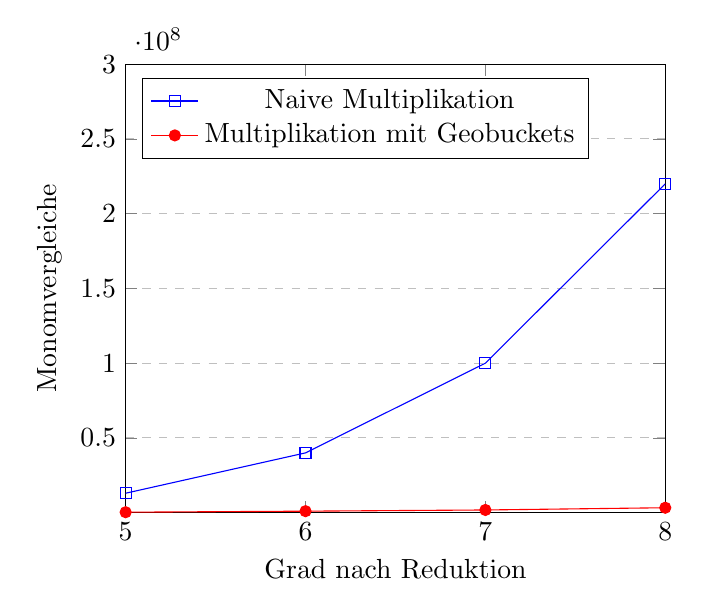
\begin{tikzpicture}
    \begin{axis}[
        xlabel={Grad nach Reduktion},
        ylabel={Monomvergleiche},
        xmin=5, xmax=8,
        ymin=100000, ymax=300000000,
        xtick={5,6,7,8},
        legend pos=north west,
        ymajorgrids=true,
        grid style=dashed,
    ]
    \addplot[
        color=blue,
        mark=square
        ]
        coordinates {
        (5, 13000000)(6, 40000000 )(7, 100000000)(8, 220000000)
        };
        \addlegendentry{Naive Multiplikation}
        
    \addplot[
        color=red,
        mark=*
        ]
        coordinates {
        (5, 300000)(6, 1000000 )(7, 1800000)(8, 3300000)
        };
        \addlegendentry{Multiplikation mit Geobuckets}
    
    \end{axis}
    \end{tikzpicture}
    \label{fig:my_label}
    \caption{Naive Multiplikation gegen Multiplikation mit Geobuckets}
\end{figure}





\begin{algorithm}
\SetAlgoLined
\label{algo:mult}
\SetKwInOut{Input}{input}
\Input{Polynome $p_1, p_2$}
// Initialize \\
$n \gets \#p_1, m\gets \#p_2$ \;
$p \gets [\ ]$ \;
Allocate $buckets$ with space for polynomials: $\{2m, 4m, ..., 2^{\lceil log_2(n)\rceil -1 }m\}$\;
$i\gets 0 $\;
// Main Loop \\
\While{$i < n$}{
    $p \gets p_1[i] \cdot p_2$\;
    \uIf{$i < (n-1)$}{
        $p \gets p + p_1[i+1] \cdot p_2$\;
    }
    $i\gets i+2$\;
   $j\gets 0 $\; 
    \While{$buckets[j].not\_empty()$}{
        $p \gets p + buckets[j]$ \;
        $buckets[j] \gets [\ ]$\;
        $j\gets j+1 $\; 
    }
    \uIf{$i < n$}{
        $buckets[j] \gets p$\;
        $p \gets [\ ]$ \;
    }
    
}
// Merge each bucket into the final polynomial\\
\ForEach{$bucket \in buckets$}{
    $p \gets p + bucket$\;
}


\Return $p$

 \caption{Polynommultipliaktion mit Geobuckets}
\end{algorithm}
